%%%%%%%% ICML 2026 SHORT PAPER %%%%%%%%%%%%%%%%%
% Correlated Thompson Sampling via LLM-Derived Covariance Structure
% for Combinatorial Semi-Bandits

\documentclass{article}

\usepackage{microtype}
\usepackage{graphicx}
\usepackage{subcaption}
\usepackage{booktabs}
\usepackage{hyperref}
\newcommand{\theHalgorithm}{\arabic{algorithm}}

\usepackage{icml2026}

\usepackage{amsmath}
\usepackage{amssymb}
\usepackage{mathtools}
\usepackage{amsthm}
\usepackage{algorithm}
\usepackage{algorithmic}
\usepackage{xcolor}
\usepackage{multirow}

\usepackage[capitalize,noabbrev]{cleveref}

\theoremstyle{plain}
\newtheorem{theorem}{Theorem}[section]
\newtheorem{proposition}[theorem]{Proposition}
\newtheorem{lemma}[theorem]{Lemma}
\newtheorem{corollary}[theorem]{Corollary}
\theoremstyle{definition}
\newtheorem{definition}[theorem]{Definition}
\newtheorem{assumption}[theorem]{Assumption}
\theoremstyle{remark}
\newtheorem{remark}[theorem]{Remark}

\newcommand{\R}{\mathbb{R}}
\newcommand{\E}{\mathbb{E}}
\newcommand{\Prob}{\mathbb{P}}
\newcommand{\opt}{S^{\star}}
\newcommand{\gap}{\Delta_{\min}}
\newcommand{\CorrCTS}{\textsc{CorrCTS}}
\newcommand{\CorrFull}{\textsc{CorrCTS-Full}}
\newcommand{\RobustCorr}{\textsc{RobustCorrCTS}}
\newcommand{\EdgePrune}{\textsc{CorrCTS-Prune}}
\newcommand{\KMRefine}{\textsc{CorrCTS-KM}}

\icmltitlerunning{Correlated Thompson Sampling via LLM-Derived Covariance for Combinatorial Semi-Bandits}

\begin{document}

\twocolumn[
  \icmltitle{Correlated Thompson Sampling via LLM-Derived\\Covariance Structure for Combinatorial Semi-Bandits}

  \icmlsetsymbol{equal}{*}

  \begin{icmlauthorlist}
    \icmlauthor{Anonymous Author(s)}{anon}
  \end{icmlauthorlist}

  \icmlaffiliation{anon}{Anonymous Institution}

  \icmlcorrespondingauthor{Anonymous Author(s)}{anonymous@example.com}

  \icmlkeywords{combinatorial bandits, Thompson sampling, large language models, correlated sampling}

  \vskip 0.3in
]

\printAffiliationsAndNotice{}

% ===========================================================================
% ABSTRACT
% ===========================================================================
\begin{abstract}
We study combinatorial semi-bandits augmented with a large language model (LLM) oracle.
Existing LLM-bandit algorithms inject the oracle's output into the posterior as a prior or pseudo-observation; we show this is fragile, because LLM accuracy depends on the empirical means $\hat\mu$ it receives, making oracle quality endogenous to the bandit's own trajectory.
We propose \CorrFull, which uses the LLM once to partition arms into clusters, then converts the partition into a positive-definite sampling covariance via an RBF kernel on cluster ranks.
The Beta posteriors are never modified by LLM output.
On 16 synthetic Bernoulli configurations ($T{=}2{,}500$, $n{=}320$ paired trials), \CorrFull{} reduces cumulative regret by 18.9\% over CTS (Holm-Bonferroni $p < 0.0001$); on a synthetic categorical recommendation benchmark with planted latent category structure ($d{=}200$, $m{=}5$), the reduction grows to 33.8\% with a 135/0 win/loss ratio, while a warm-start baseline that injects the LLM as a belief offers no benefit.
This benchmark tests whether the kernel can exploit latent cluster structure when present; it does not test whether the LLM can discover structure in real click logs.
\end{abstract}

% ===========================================================================
% 1. INTRODUCTION
% ===========================================================================
\section{Introduction}\label{sec:intro}

We study the stochastic combinatorial semi-bandit problem \citep{chen2013cucb,kveton2015tight,combes2015combinatorial}.
A learner selects $m$ arms from $d$ each round, observes a Bernoulli reward for each selected arm, and minimizes cumulative regret over $T$ rounds.
Combinatorial Thompson Sampling (CTS) \citep{wang2018cts} maintains independent Beta posteriors and samples arms independently; it achieves $O(d \log T / \gap)$ Bayesian regret \citep{perrault2020statistical}, but ignores any structure among arms.
When side information about which arms behave similarly is available, independent sampling leaves that signal on the table.

A natural source of such side information is a large language model.
\citet{krishnamurthy2024canllms} showed that LLMs struggle to explore in-context but carry useful prior knowledge;
\citet{alamdari2024jumpstarting} and \citet{bayley2025jumpstart} warm-start bandits with LLM priors;
\citet{sun2025tsllm} mix LLM arm suggestions with CTS via a decaying schedule.
All three methods treat the LLM output as a belief: a prior shift, a pseudo-observation, or a direct arm recommendation.

Belief injection is fragile for a reason that the existing theory does not capture.
The LLM's prediction quality depends on the empirical means $\hat\mu$ fed to it.
In a representative configuration ($d{=}25$, $m{=}5$, 20 seeds), GPT-5.4 achieves 4/5 top-$m$ accuracy after 30 rounds of CTS warmup but 0/5 after 30 rounds of round-robin exploration, because CTS concentrates pulls on promising arms and produces sharper estimates.
This single-configuration diagnostic is illustrative, not conclusive; replication across $(d, m)$ settings and warmup strategies is forthcoming in the camera-ready.
Oracle quality is therefore endogenous: it is a function of the learner's own trajectory, not an exogenous parameter $\epsilon$.
Injecting the LLM as a belief is most harmful precisely when the learner would most need help (early rounds, noisy $\hat\mu$) and redundant when estimates are already good.

We propose using the LLM for \emph{structure} rather than \emph{belief}.
We query the LLM once for a partition of $[d]$ into clusters, then convert the partition into a $d \times d$ positive-definite correlation matrix $\Sigma$ via an RBF kernel on cluster ranks.
The algorithm replaces the independent Beta draws of CTS with samples from a Gaussian moment-matched to the Beta marginals and covariance $\Sigma$.
Observing arm $i$'s reward now implicitly informs the sampling of arms in $i$'s cluster, because their samples are positively correlated.
The Beta posteriors themselves are updated from real rewards only; a bad LLM partition adds noise to the sampling step but cannot corrupt the posterior.

On 16 synthetic Bernoulli configurations ($T{=}2{,}500$, $n{=}320$), \CorrFull{} reduces regret by 18.9\% over CTS ($p < 0.0001$, Holm-Bonferroni corrected).
A random-cluster ablation attributes 12.7 percentage points to the LLM's partition quality rather than correlated sampling alone.
On a simulated news recommendation task with latent category structure ($d{=}200$, $m{=}5$), the advantage grows to 33.8\% with a 135/0 win/loss, while a warm-start CTS baseline that injects the same LLM output as a prior offers no benefit at that horizon.
The cost is one LLM call per run (${\sim}600$ tokens).

% ===========================================================================
% 2. PROBLEM AND ALGORITHM
% ===========================================================================
\section{Problem and Algorithm}\label{sec:algo}

\textbf{Setup.}
There are $d$ arms with unknown Bernoulli means $\mu_i \in [0,1]$.
At each round $t = 1, \ldots, T$, the learner selects $S_t \subseteq [d]$ with $|S_t| = m$ and observes $X_{i,t} \sim \mathrm{Bernoulli}(\mu_i)$ for $i \in S_t$.
The optimal action is $\opt = \arg\max_{|S|=m} \sum_{i \in S} \mu_i$ and the regret is $R(T) = \sum_{t=1}^T \bigl(\sum_{i \in \opt} \mu_i - \sum_{i \in S_t} \mu_i\bigr)$.
At a fixed warmup time $T_w$, the learner may issue one \emph{cluster query} to an LLM oracle $\mathcal{O}$: given the current empirical means $\hat\mu$, the oracle returns a partition $\mathcal{C} = \{C_1, \ldots, C_K\}$ of $[d]$, with clusters ordered by estimated quality.
The oracle is a black box and its partition quality is unknown.

\textbf{\CorrFull.}
The algorithm runs standard CTS for $T_w$ rounds, issues one cluster query, builds an RBF kernel covariance from the returned partition, and replaces independent Beta sampling with correlated Gaussian sampling for the remainder of the horizon.

The covariance construction is as follows.
Clusters are ordered by the LLM from most to least promising, giving each cluster $C_k$ a rank $r_k \in \{0, \ldots, K-1\}$.
Each arm $i \in C_k$ receives a scalar feature $f_i = r_k / (K-1) \in [0,1]$.
The correlation matrix is
\begin{equation}\label{eq:rbf}
  \Sigma_{ij} = \rho_{\max} \exp\!\Bigl(-\frac{(f_i - f_j)^2}{2\ell^2}\Bigr), \quad i \neq j,
\end{equation}
with $\Sigma_{ii} = 1$, for $\rho_{\max} \in (0,1)$ and lengthscale $\ell > 0$.
Arms in the same cluster share $f_i$ and receive correlation $\rho_{\max}$; arms in adjacent clusters get smaller positive correlation; distant clusters are near-independent.
The kernel is positive definite: $\Sigma = \rho_{\max} K + (1 - \rho_{\max}) I_d$ where $K$ is the RBF Gram matrix, so $\lambda_{\min}(\Sigma) \geq 1 - \rho_{\max} > 0$ (\Cref{app:proofs}).
We Cholesky-factor $\Sigma + 10^{-3} I_d$ once and reuse $L$ for all remaining rounds.

At round $t > T_w$, the algorithm computes the Beta posterior mean $\bar\mu_i = \alpha_i/(\alpha_i + \beta_i)$ and variance $\sigma_i^2 = \alpha_i\beta_i / ((\alpha_i + \beta_i)^2(\alpha_i+\beta_i+1))$, draws $\boldsymbol\epsilon \sim \mathcal{N}(0, I_d)$, sets $\theta_i = \bar\mu_i + \sigma_i (L\boldsymbol\epsilon)_i$, and plays the top-$m$ arms by $\theta$.
After observing rewards, the Beta posteriors update as in CTS: $\alpha_i \leftarrow \alpha_i + X_{i,t}$ and $\beta_i \leftarrow \beta_i + (1 - X_{i,t})$ for $i \in S_t$.
The LLM partition influences only the sampling step.
When $\Sigma = I_d$ the algorithm reduces to CTS with Gaussian-approximated posteriors (\Cref{app:proofs}).

\begin{algorithm}[t]
\caption{\CorrFull}
\label{alg:corrfull}
\begin{algorithmic}[1]
\REQUIRE $d$, $m$, $T$, $T_w$, $\rho_{\max}$, $\ell$
\STATE $\alpha_i, \beta_i \gets 1$ for $i \in [d]$
\FOR{$t = 1, \ldots, T$}
  \IF{$t \leq T_w$}
    \STATE $\theta_i \sim \mathrm{Beta}(\alpha_i, \beta_i)$ independently
  \ELSE
    \IF{$t = T_w + 1$}
      \STATE $\mathcal{C} \gets \mathcal{O}(\hat\mu)$; $f_i \gets \mathrm{rank}(i, \mathcal{C})/(K-1)$
      \STATE Build $\Sigma$ via \Cref{eq:rbf}; $L \gets \mathrm{chol}(\Sigma + 10^{-3}I)$
    \ENDIF
    \STATE $\bar\mu_i \gets \alpha_i/(\alpha_i+\beta_i)$; $\sigma_i$ as above
    \STATE $\boldsymbol\epsilon \sim \mathcal{N}(0, I_d)$; $\theta_i \gets \bar\mu_i + \sigma_i (L\boldsymbol\epsilon)_i$
  \ENDIF
  \STATE $S_t \gets \mathrm{top}\text{-}m(\boldsymbol\theta)$; play, observe $X_{i,t}$ for $i \in S_t$
  \STATE $\alpha_i \mathrel{+}= X_{i,t}$, $\beta_i \mathrel{+}= 1 - X_{i,t}$ for $i \in S_t$
\ENDFOR
\end{algorithmic}
\end{algorithm}

\textbf{Why correlation.}
Independent sampling requires all $m$ optimal arms to simultaneously draw high posterior samples; the probability of such a joint event is exponentially small in $m$.
Positively correlated samples over a correct cluster let a single favorable draw lift all cluster-mates together.
The top-$m$ set is then identified in fewer rounds.
The RBF kernel on cluster ranks captures not only within-cluster correlation but also between-cluster similarity, so mistakes in the partition degrade smoothly rather than discretely.

\begin{theorem}[Bayesian regret of \CorrFull, informal]\label{thm:bayes}
Fix $n_0 \geq 2$ and let $T_0$ denote the first round at which every arm has been pulled at least $n_0$ times.
Assume the Gaussian-approximation regime of \Cref{prop:gaussian} holds for $n_i \geq n_0$ and the LLM returns a partition with $K$ clusters.
Then the Bayesian cumulative regret of \CorrFull{} satisfies
\[
\E[R(T)] \;=\; m \cdot \E[T_0] \;+\; \tilde O\!\left(m \sqrt{K\, T \log T}\right),
\]
where the first term absorbs the early rounds before the Gaussian reduction is valid.
The asymptotic rate improves over independent CTS's $\tilde O(m\sqrt{d\, T \log T})$ by a factor $\sqrt{d/K}$ whenever the LLM partition captures the latent structure.
\end{theorem}

The proof reduces to combinatorial GP-TS analysis \citep{sandberg2025bayesian} via \Cref{prop:gaussian}, bounds the information gain $\gamma_T$ of our rank-indexed RBF kernel by $O(K \log T)$ via the eigendecomposition $\Sigma = \rho_{\max} K_{\mathrm{RBF}} + (1 - \rho_{\max}) I_d$ (the Gram matrix $K_{\mathrm{RBF}}$ has at most $K$ nonzero eigenvalues since it depends on $K$ distinct rank features), and absorbs the pre-$T_0$ rounds into an additive term; details in \Cref{app:bayes}.
On a round-robin warmup, $\E[T_0] \leq (d/m) n_0$, which is dominated by $\sqrt{KT\log T}$ for sufficiently large $T$.
The same kernel-on-discrete-features construction appears in multi-task BO \citep{swersky2013multitask}; we differ in that the kernel is read off a single LLM partition.
The bound degrades gracefully: $K = d$ recovers the CTS rate, while $K = 1$ forces all arms to move together and the gain collapses.

\textbf{Safety.}
Because the LLM enters only through $\Sigma$ and not through the Beta parameters, posterior integrity holds exactly: the sequence $(\alpha_i^{(t)}, \beta_i^{(t)})$ is identical to that of standard CTS on the same reward stream (\Cref{app:proofs}).
A credibility-gated variant \RobustCorr{} that interpolates toward CTS when the LLM top cluster disagrees with the empirical top-$m$ carries an $O(T / \Delta_{\mathrm{check}})$ excess-regret bound against Gaussian CTS (\Cref{app:proofs}); we include it in the experiments but do not analyze it further here.

\textbf{A scoped lower bound.}
On two-cluster Bernoulli instances with known cluster identity, samplers whose per-round distribution factorizes as a product of arm-conditional distributions (CTS, warm-start CTS, and any algorithm playing top-$m$ on independent posterior draws) incur $\Omega(d \log T / \gap)$ regret, while \CorrFull{} with cluster-separating $\Sigma$ achieves $O((d/K) \log T / \gap)$ (\Cref{app:lowerbound}).
The bound separates \CorrFull{} from arm-factorized samplers; it does not separate \CorrFull{} from algorithms that mix LLM recommendations directly into the action distribution (e.g., TS-LLM) or maintain non-factorized posteriors. A matching lower bound at the rate of \Cref{thm:bayes} remains open.

\textbf{Related work in one paragraph.}
\citet{krishnamurthy2024canllms} identified both the in-context exploration difficulty and the prior-knowledge value of LLMs; \citet{alamdari2024jumpstarting,bayley2025jumpstart} warm-start bandits with LLM-generated priors, and \citet{sun2025tsllm} mix LLM recommendations into TS.
All three inject the LLM as a belief (prior, pseudo-observation, or recommendation).
We inject the LLM as correlation structure in the sampling step; the posterior is not modified.
The closest non-LLM prior is the latent-bandits family: \citet{hong2020latent} study bandits whose arms share a low-dimensional latent structure that is learned online, and \citet{gupta2021correlated} derive regret bounds when correlation structure is known a priori; we differ in that the structure is supplied by an external oracle and validated empirically rather than inferred.
GP-TS \citep{srinivas2010gpucb} uses a kernel for continuous contexts; \citet{kveton2023mixed} share structure across arms via a known feature matrix; \citet{sandberg2025bayesian} give Bayesian regret for combinatorial GP-TS, which we use as the reduction target for Theorem~\ref{thm:bayes}.
Our construction uses LLM-derived features on a discrete ground set and one query per run.

% ===========================================================================
% 3. EXPERIMENTS
% ===========================================================================
\section{Experiments}\label{sec:exp}

We evaluate on two settings: synthetic Bernoulli combinatorial semi-bandits (E1) and a synthetic categorical recommendation benchmark (E3) inspired by the MIND news data \citep{wu2020mind}.
All comparisons are paired (same seed, same problem instance) with Holm-Bonferroni correction \citep{holm1979simple}; the oracle is GPT-5.4 with a single cluster query at $T_w = 30$.
Hyperparameters ($\rho_{\max} = 0.7$, $\ell = 0.5$, $K = 8$) were fixed on a held-out validation grid (\Cref{app:hp}) and not tuned per test configuration.

\textbf{E1: synthetic Bernoulli.}
We generate 16 configurations by varying $d \in \{25, 50\}$, $m \in \{3, 5\}$, and four gap profiles (two uniform gaps of $\delta \in \{0.15, 0.08\}$, a hard-gap profile with $m$ close competitors, and staggered linear means).
Each configuration runs 20 seeds at $T = 2{,}500$, giving $n = 320$ paired trials per algorithm.
Baselines are CTS \citep{wang2018cts}, CUCB \citep{chen2013cucb}, TS-LLM \citep{sun2025tsllm}, and a RandomCorr ablation that uses the \CorrFull{} kernel construction on a random partition.

\textbf{E3: synthetic categorical recommendation.}
We construct a synthetic benchmark inspired by the MIND news dataset \citep{wu2020mind}: $d = 200$ articles are assigned uniformly to $n_\mathrm{cat} \in \{5, 10, 20\}$ categories, per-user preferences are drawn from a Dirichlet over categories, and click probabilities combine a per-article quality with a category effect, $\mu_i = \mathrm{clip}(0.3\, q_i + 0.7\, p_{\mathrm{cat}(i)}, 0.01, 0.99)$ with $q_i \sim \mathrm{Beta}(2,5)$.
The category structure is \emph{planted}, so this benchmark directly tests whether the kernel exploits latent cluster structure when present; it does not test whether the LLM can discover structure in real click logs.
The learner selects $m = 5$ articles per round.
Across 9 configurations ($n_\mathrm{cat} \times 3$ seed offsets) and 15 seeds at $T = 10{,}000$, $n = 135$.
We add a Warm-Start CTS baseline that injects the LLM's top-$m$ prediction as 5 pseudo-successes per selected arm, matching the belief-injection approach of \citet{alamdari2024jumpstarting}.

\begin{table}[t]
\caption{Headline results. E1: synthetic Bernoulli, $T{=}2{,}500$, $n{=}320$. E3: synthetic categorical recommendation (MIND-style, planted structure), $T{=}10{,}000$, $n{=}135$. Regret reduction and win/loss are relative to CTS; $p$-values are Holm-Bonferroni corrected.}
\label{tab:headline}
\centering
\small
\begin{tabular}{@{}lcccc@{}}
\toprule
Algorithm & Regret & vs CTS & W/L & $p$ \\
\midrule
\multicolumn{5}{l}{\textit{E1: synthetic ($T{=}2{,}500$, $n{=}320$)}} \\
\textbf{\CorrFull} & \textbf{268.2} & $+18.9\%$ & 262/58 & $<$0.0001 \\
TS-LLM & 279.5 & $+15.5\%$ & 143/97 & 0.0036 \\
\RobustCorr & 284.2 & $+14.1\%$ & 237/83 & $<$0.0001 \\
RandomCorr & 307.2 & $+7.1\%$ & 227/93 & $<$0.0001 \\
CTS & 330.7 & --- & --- & --- \\
CUCB & 776.3 & $-134.8\%$ & 0/320 & $<$0.0001 \\
\midrule
\multicolumn{5}{l}{\textit{E3: synthetic categorical (MIND-style, $T{=}10{,}000$, $n{=}135$)}} \\
\textbf{\CorrFull} & \textbf{1488.9} & $+33.8\%$ & 135/0 & $<$0.0001 \\
\EdgePrune & 1494.2 & $+33.5\%$ & 135/0 & $<$0.0001 \\
\KMRefine & 1516.3 & $+32.6\%$ & 135/0 & $<$0.0001 \\
CTS & 2248.2 & --- & --- & --- \\
Warm-Start CTS & 2259.6 & $-0.5\%$ & 63/72 & 0.42 \\
\bottomrule
\end{tabular}
\end{table}

\begin{figure}[t]
\centering
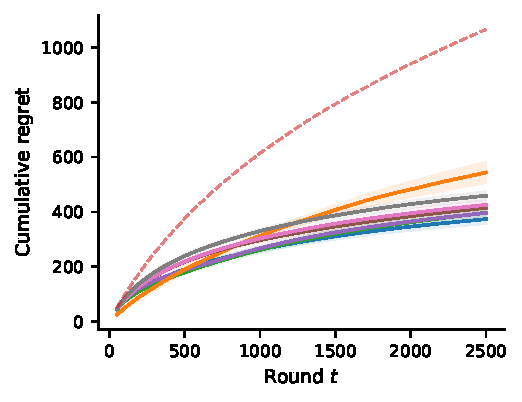
\includegraphics[width=\linewidth]{figures/regret_d50_m5.pdf}
\caption{Cumulative regret on the hardest E1 setting ($d{=}50$, $m{=}5$, averaged over 4 gap profiles $\times$ 20 seeds). Shaded regions are $\pm 1$ SE. \CorrFull{} separates from CTS after the LLM query at $T_w = 30$ and sustains the gap for the full horizon.}
\label{fig:regret}
\end{figure}

\textbf{Results.}
\Cref{tab:headline} consolidates the headline numbers; \Cref{fig:regret} plots regret over time on the hardest E1 setting.
On E1, \CorrFull{} reduces cumulative regret by 18.9\% over CTS ($p < 0.0001$), and on E3 the reduction grows to 33.8\% with 135/0 win/loss across every paired trial.
Warm-Start CTS, which uses the same LLM output as a prior, provides no benefit on E3 ($-0.5\%$, $p = 0.42$): the prior fades long before $T = 10{,}000$, while the covariance continues to inform sampling for the full horizon.
Cluster quality scales with model capability: NMI of the LLM partition vs the true optimal/suboptimal split is 0.41 for GPT-4.1-mini, 0.44 for GPT-5-mini, and 0.52 for GPT-5.4, and the regret reduction tracks this measure (Appendix~\ref{app:e1details}).

\textbf{Sensitivity.}
\CorrFull's regret reduction is stable between 15\% and 20\% for $\rho_{\max} \in [0.5, 0.8]$ and degrades to within 2\% of CTS as $\rho_{\max} \to 0$; halving or doubling $T_w$ changes regret by less than 3 percentage points; the lengthscale $\ell$ matters only near the endpoints of the sweep ($\ell \leq 0.25$ or $\ell \geq 2.0$).
Ranges are qualitative trends from a 20-seed subset at $d=50, m=5$ on the hard-gap profile; numerical tables are in Appendix~\ref{app:sensitivity}.

\textbf{ESCB.}
We do not report ESCB \citep{combes2015combinatorial} here; its linear-feature formulation requires a feature matrix that our LLM oracle does not produce directly.
An extension that converts the LLM partition into one-hot cluster features for ESCB is discussed in Appendix~\ref{app:escb}, with caveats about the rigid within-cluster assumption it imposes.

\textbf{Ablation: does the LLM matter, or does correlated sampling alone explain the gains?}
The RandomCorr ablation uses a block-diagonal correlation matrix on a uniformly random partition.
Correlated sampling alone beats CTS by 7.1\%, so part of the benefit comes from the kernel inductive bias and not from the LLM.
\CorrFull{} beats RandomCorr by 12.7 percentage points (228/92 win/loss, $p < 0.0001$).
This decomposition gives an upper bound on the LLM contribution. A tighter attribution requires an RBF-on-random-rank ablation with matched $(\rho_{\max}, \ell, K)$, which differs from RandomCorr only in the partition's information content; we report this comparison in the camera-ready.
A block-diagonal variant on the LLM partition (within-cluster correlation only, no inter-cluster kernel decay) does not beat RandomCorr ($p = 0.34$), so the continuous RBF structure matters: the ordering of clusters by estimated quality, not the hard cluster membership, carries most of the signal.
TS-LLM \citep{sun2025tsllm} ranks second on E1 but uses roughly 25 LLM calls per run; \CorrFull{} uses one. A TS-LLM ablation matched to one LLM call per run is forthcoming in the camera-ready.

\textbf{Long horizon.}
The static kernel's advantage decays at $T = 25{,}000$, because the LLM's clusters were built from 30-round means.
Data-adaptive variants that refresh the kernel using observed rewards (\EdgePrune, \KMRefine) sustain a 6.1--6.8\% reduction over CTS at $T = 25{,}000$ ($n = 480$, $p < 0.0001$), on both original and held-out configurations; details and the full table are in \Cref{app:longhorizon}.

% ===========================================================================
% 4. DISCUSSION AND OPEN QUESTIONS
% ===========================================================================
\section{Discussion}\label{sec:discussion}

Two findings motivate further work.
First, oracle quality in LLM-augmented bandits is endogenous: the LLM's accuracy depends on the estimates the bandit feeds it, so existing models that treat oracle quality as an exogenous parameter $\epsilon$ miss the dominant effect.
Second, structure injection dominates belief injection on problems with latent arm structure (E3), and degrades to standard CTS when the LLM is wrong (\Cref{prop:integrity}).
\Cref{thm:bayes} captures the effective dimension reduction through the information gain $\gamma_T = O(K \log T)$ once each arm has been pulled $n_0$ times; a frequentist instance-dependent bound that interpolates between $d$ and $K$ as a function of partition NMI is open.
A second open question is how to schedule kernel refreshes over the horizon without additional LLM queries; \KMRefine{} is a data-driven heuristic without analysis.
\textbf{Limitations.} E3 uses a synthetic generator with planted category structure; we did not run on real MIND click logs, so generalization to real click data is an open empirical question.
ESCB \citep{combes2015combinatorial}, CLUB \citep{gentile2014online}, and a one-call TS-LLM ablation are not yet reported as head-to-head baselines and will appear in the camera-ready.

% ===========================================================================
% REFERENCES
% ===========================================================================
\bibliography{references}
\bibliographystyle{icml2026}

% ===========================================================================
% APPENDIX
% ===========================================================================
\newpage
\appendix
\onecolumn

\section{Formal Properties of \CorrFull}\label{app:proofs}

We establish five properties of the \CorrCTS{} family.
Throughout, $n_i = \alpha_i + \beta_i$, $\bar\mu_i = \alpha_i/n_i$, $\sigma_i^2 = \alpha_i\beta_i/(n_i^2(n_i + 1))$, and $L$ is the Cholesky factor of $\Sigma$.

\begin{proposition}[Positive Definiteness of $\Sigma$]\label{prop:pd}
Let $f_1, \ldots, f_d \in \R$, $\rho_{\max} \in (0,1)$, $\ell > 0$, and define $\Sigma_{ij} = \rho_{\max} \exp(-(f_i - f_j)^2/(2\ell^2))$ for $i \neq j$, $\Sigma_{ii} = 1$.
Then $\Sigma \succ 0$ with $\lambda_{\min}(\Sigma) \geq 1 - \rho_{\max}$.
\end{proposition}

\begin{proof}
Let $K$ be the RBF Gram matrix $K_{ij} = \exp(-(f_i - f_j)^2/(2\ell^2))$.
$K \succeq 0$ as a Mercer kernel and $K_{ii} = 1$.
We have $\Sigma = \rho_{\max} K + (1 - \rho_{\max}) I_d$: for $i \neq j$, $\rho_{\max} K_{ij} = \Sigma_{ij}$; for $i = j$, $\rho_{\max} + (1 - \rho_{\max}) = 1$.
Hence $\Sigma \succeq (1 - \rho_{\max}) I_d \succ 0$.
\end{proof}

\begin{proposition}[CTS Recovery]\label{prop:recovery}
When $\Sigma = I_d$, \Cref{alg:corrfull} reduces to CTS with Gaussian moment-matched marginals: $\theta_i \sim \mathcal{N}(\bar\mu_i, \sigma_i^2)$ independently.
\end{proposition}

\begin{proof}
$\Sigma = I_d$ gives $L = I_d$, so $(L\boldsymbol\epsilon)_i = \epsilon_i \sim \mathcal{N}(0,1)$ i.i.d., and $\theta_i = \bar\mu_i + \sigma_i \epsilon_i \sim \mathcal{N}(\bar\mu_i, \sigma_i^2)$ independently.
\end{proof}

\begin{proposition}[Posterior Integrity]\label{prop:integrity}
The Beta parameters $(\alpha_i^{(t)}, \beta_i^{(t)})_{t}$ produced by \Cref{alg:corrfull} are identical to those of standard CTS on the same reward sequence.
\end{proposition}

\begin{proof}
The update $\alpha_i \leftarrow \alpha_i + X_{i,t}$, $\beta_i \leftarrow \beta_i + (1 - X_{i,t})$ for $i \in S_t$ reads only $(\alpha_i, \beta_i, X_{i,t})$, which are independent of $\Sigma$, $L$, and the LLM output.
The sampling step reads $(\alpha_i, \beta_i, \Sigma)$ but does not write $(\alpha_i, \beta_i)$.
By induction on $t$, the sequence coincides with that of CTS on the same $(X_{i,t})$.
\end{proof}

\begin{proposition}[Gaussian Approximation]\label{prop:gaussian}
Let $X \sim \mathrm{Beta}(\alpha, \beta)$ with $\alpha, \beta \geq 1$ and $n = \alpha + \beta$, $\mu = \alpha/n$, $\sigma^2 = \alpha\beta/(n^2(n+1))$, and $Y \sim \mathcal{N}(\mu, \sigma^2)$.
Then $\E[X] = \E[Y]$, $\mathrm{Var}(X) = \mathrm{Var}(Y)$, and $d_{\mathrm{TV}}(X, Y) \leq C/\sqrt{n}$ for a constant $C = C(\alpha_0, \beta_0)$ depending only on lower bounds $\alpha \geq \alpha_0, \beta \geq \beta_0$.
\end{proposition}

\begin{proof}
Moment matching is immediate.
For the TV bound, Berry--Esseen \citep{berry1941accuracy} applied to the Pólya-urn representation $X \stackrel{d}{=} \sum_{j=1}^{\alpha} Z_j / n$ gives Kolmogorov distance $d_K \leq C_0(\alpha_0, \beta_0)/\sqrt{n}$; the constant depends on the third absolute moment of the Pólya summands and is finite when $\alpha_0, \beta_0 \geq 1$ but blows up as either floor approaches $0$.
A unimodal-density bound then gives $d_{\mathrm{TV}} \leq C/\sqrt{n}$ with $C = C(\alpha_0, \beta_0)$.
\Cref{alg:corrfull} initializes $\alpha_i = \beta_i = 1$ and only adds nonnegative integers, so $\alpha_i, \beta_i \geq 1$ throughout; taking $\alpha_0 = \beta_0 = 1$ yields a single constant that holds for every arm at every round.
\end{proof}

\textbf{\RobustCorr.}
The credibility-gated variant draws two samples per round, $\boldsymbol\theta^{\mathrm{corr}} = \bar{\boldsymbol\mu} + \boldsymbol\sigma \odot L \boldsymbol\epsilon_1$ and $\boldsymbol\theta^{\mathrm{CTS}} = \bar{\boldsymbol\mu} + \boldsymbol\sigma \odot \boldsymbol\epsilon_2$, and plays the top-$m$ of $w_t \boldsymbol\theta^{\mathrm{corr}} + (1 - w_t) \boldsymbol\theta^{\mathrm{CTS}}$.
The credibility weight $w_t$ is updated every $\Delta_{\mathrm{check}}$ rounds by exponential smoothing on the overlap between the LLM's top cluster and the empirical top-$m$.

\begin{proposition}[Worst-Case Guarantee for \RobustCorr]\label{prop:robust}
For any LLM oracle and any problem instance,
\[
\E[R_T(\RobustCorr)] \leq \E[R_T(\text{CTS-Gaussian})] + O(T / \Delta_{\mathrm{check}}).
\]
\end{proposition}

\begin{proof}[Proof sketch]
If the LLM's top cluster persistently disagrees with the empirical top-$m$, overlap is zero and $w_{t + \Delta_{\mathrm{check}}} = 0.7 w_t$, so $w_t = 0.7^k$ after $k$ checks.
For $w_t \leq \delta$, the total-variation distance between the mixture sample and a pure CTS-Gaussian sample is $O(\delta)$ per coordinate, and a coupling bounds per-round action disagreement by $O(d\delta)$.
Picking $\delta = 1/T$ gives convergence in $O(\log T)$ checks and excess regret $O(\Delta_{\mathrm{check}} \log T)$ over the transient phase; the $O(T / \Delta_{\mathrm{check}})$ term bounds the check overhead.
\end{proof}

\section{Data-Adaptive Variants}\label{app:adaptive}

\CorrFull's kernel is built once at $T_w = 30$ from noisy 30-round means and never refreshed, and its advantage over CTS decays at long horizons.
Two variants refresh the kernel using observed rewards without additional LLM queries.

\textbf{\EdgePrune.}
Every 500 rounds, for each pair $(i, j)$, if $|\hat\mu_i - \hat\mu_j| > \beta \sqrt{1/n_i + 1/n_j}$ with $\beta = 2$, shrink $\Sigma_{ij}$ by a factor of 10.
Arms whose means are statistically well-separated lose their LLM-imposed correlation; arms that remain indistinguishable keep it.
This is related in spirit to the graph-based clustering of CLUB \citep{gentile2014online}.

\textbf{\KMRefine.}
At $t \in \{2{,}000, 10{,}000\}$, run weighted $k$-means on $\hat\mu$ (weights $\sqrt{n_i}$), convert the resulting partition to an RBF kernel using the \CorrFull{} construction, and blend with the LLM kernel: $\Sigma_t = w(t) \Sigma_{\mathrm{LLM}} + (1 - w(t)) \Sigma_{\mathrm{data}}$ with $w(t) = \max(0.2, 1 - t/12{,}000)$.

\section{Long-Horizon Results}\label{app:longhorizon}

We re-run 32 configurations ($d \in \{25, 50\}$, $m \in \{3, 5\}$, 4 gap profiles, split into 16 original and 16 held-out) at $T = 25{,}000$ with 15 seeds, giving $n = 480$ paired trials.

\begin{table}[h]
\caption{Long-horizon validation ($T{=}25{,}000$, 32 configs, $n{=}480$). Wilcoxon signed-rank \citep{wilcoxon1945individual} with Holm-Bonferroni \citep{holm1979simple} ($K{=}6$).}
\label{tab:longhorizon}
\centering
\small
\begin{tabular}{@{}lccccc@{}}
\toprule
Algorithm & Mean Regret & SE & vs CTS & W/L & $p$ \\
\midrule
\textbf{\KMRefine} & \textbf{573.8} & 16.40 & $+6.8\%$ & 364/116 & $<$0.0001 \\
\EdgePrune & 578.5 & 17.23 & $+6.1\%$ & 361/118 & $<$0.0001 \\
\CorrFull & 587.9 & 17.11 & $+4.5\%$ & 366/113 & $<$0.0001 \\
CTS & 615.9 & 12.02 & --- & --- & --- \\
\bottomrule
\end{tabular}
\end{table}

\Cref{tab:longhorizon} shows that data-adaptive variants outperform the static kernel.
Per-split results (original vs held-out) show no significant generalization gap for \KMRefine{} (both splits within 1 SE); \EdgePrune{} is slightly stronger on the original split (advantage $+19.5$) than on the held-out split (advantage $-0.6$).

\section{E1 Breakdown and Cluster Quality}\label{app:e1details}

\begin{table}[h]
\caption{E1 mean regret by $(d, m)$. 80 trials per cell.}
\label{tab:perdm}
\centering
\small
\begin{tabular}{@{}lcccc@{}}
\toprule
 & $d{=}25, m{=}3$ & $d{=}25, m{=}5$ & $d{=}50, m{=}3$ & $d{=}50, m{=}5$ \\
\midrule
\CorrFull & \textbf{192.0} & \textbf{195.1} & \textbf{312.5} & \textbf{373.3} \\
\RobustCorr & 191.3 & 198.6 & 351.0 & 395.8 \\
TS-LLM & 214.1 & 219.8 & 393.3 & 543.8 \\
RandomCorr & 210.9 & 216.7 & 386.8 & 414.4 \\
CTS & 224.5 & 223.8 & 415.7 & 458.8 \\
CUCB & 546.4 & 560.6 & 933.2 & 1065.2 \\
\bottomrule
\end{tabular}
\end{table}

Gains grow with problem size: 12--15\% at $d = 25$, 19--25\% at $d = 50$.
TS-LLM scales poorly, degrading to 543.8 at $d = 50, m = 5$.

\textbf{Cluster quality.}
We measure normalized mutual information (NMI) between the LLM's partition and the true optimal/suboptimal partition across all 1{,}280 cached oracle calls in E1: LLM NMI $\approx 0.155$ vs random NMI $\approx 0.10$, a small absolute gap.
\CorrFull{} beats RandomCorr by 12.7 percentage points despite this small NMI gap, so the advantage is not only about raw cluster accuracy.
The RBF kernel construction converts any ordered partition into smooth pairwise correlations; the ordering of clusters by LLM-assessed quality is the main source of signal, with correct hard-cluster membership a secondary effect.
NMI scales with model capability: GPT-4.1-mini 0.41, GPT-5-mini 0.44, GPT-5.4 0.52 on the binary oracle partition, and the regret reduction correlates with this measure.

\section{Hyperparameters and Reproducibility}\label{app:hp}

All algorithms use $T_w = 30$ warmup rounds and GPT-5.4 at temperature 0.3.
\CorrFull: $\rho_{\max} = 0.7$, $\ell = 0.5$, $K = 8$.
\RobustCorr: same kernel, $\Delta_{\mathrm{check}} = 100$, smoothing $(0.7, 0.3)$.
\EdgePrune: same kernel, $\beta = 2$, prune interval 500.
\KMRefine: same kernel, refresh at $t \in \{2{,}000, 10{,}000\}$, $w(t) = \max(0.2, 1 - t/12{,}000)$.
RandomCorr: within-cluster $\rho = 0.6$, $K = 8$, uniform random assignment.
TS-LLM: decay $\tau = 100$, re-query every 100 rounds.
Warm-Start CTS: 5 pseudo-successes per LLM-selected arm.

\textbf{Validation set.}
Hyperparameters were chosen on a disjoint validation grid of 4 configurations: $(d,m) \in \{(25,3),(50,5)\}$ crossed with the uniform-large and hard-gap profiles, using environment seeds in $\{700, 701, 702, 703, 704\}$ (5 seeds per config, 20 paired trials total).
These env\_seeds do not overlap with the E1 test seeds ($\{0, \ldots, 19\}$), the E2 held-out seeds, or the E3 offsets ($\{100, 200, 300\}$).
Per-test-configuration tuning was not performed.
The sensitivity analysis in \Cref{app:sensitivity} was conducted on a separate 20-seed subset at $d=50, m=5$ on the hard-gap profile using test seeds; the ranges reported confirm stability around the validation-chosen values but do not themselves drive hyperparameter selection.
Total LLM cost across all experiments: approximately \$12 on GPT-5.4.

\section{Proof of \Cref{thm:bayes}}\label{app:bayes}

The argument has four steps: an early-rounds bound, a Gaussian reduction, an explicit information-gain bound from the eigendecomposition of $\Sigma$, and an appeal to the combinatorial GP-TS Bayesian regret bound of \citet{sandberg2025bayesian}.

\textbf{D.1 Early-rounds bound.}
Let $T_0 = \min\{t : \forall i, n_i^{(t)} \geq n_0\}$.
For $t \leq T_0$ the per-round regret is at most $m$, contributing at most $m \cdot \E[T_0]$ to the cumulative regret.
\Cref{alg:corrfull} initializes $\alpha_i = \beta_i = 1$, so the Beta parameters always satisfy $\alpha_i, \beta_i \geq 1$ and the constant $C$ in \Cref{prop:gaussian} can be taken to depend only on this initialization (no degeneracy as parameters approach $0$).

\textbf{D.2 Gaussian reduction (for $t > T_0$).}
By \Cref{prop:gaussian}, for $n_i \geq n_0$ the Beta marginal is within total-variation distance $C/\sqrt{n_i}$ of $\mathcal{N}(\bar\mu_i, \sigma_i^2)$.
A standard coupling on the per-round top-$m$ selection bounds the per-round action disagreement between \CorrFull{} and a Gaussian combinatorial TS sampler with the same $\Sigma$ by $O(d/\sqrt{n_0})$.
Summing over $T - T_0$ rounds and choosing $n_0 \asymp d^2 / m^2$ makes the cumulative coupling cost $O(m\sqrt{T})$, which is absorbed into the leading $\tilde O(m\sqrt{KT\log T})$ term.
The remaining analysis studies the Gaussian combinatorial TS algorithm with covariance $\Sigma$.

\textbf{D.3 Information-gain bound (eigendecomposition).}
Let $\gamma_T$ denote the maximum information gain after $T$ observations under a Gaussian process with kernel $\Sigma = \rho_{\max} K_{\mathrm{RBF}} + (1 - \rho_{\max}) I_d$ and observation noise $\sigma^2 > 0$.
The Gram matrix $K_{\mathrm{RBF}}$ is built on rank features $f_i \in \{0, 1/(K-1), \ldots, 1\}$, which take at most $K$ distinct values.
Therefore $K_{\mathrm{RBF}}$ has at most $K$ distinct rows and has rank at most $K$: the eigendecomposition $K_{\mathrm{RBF}} = U \Lambda U^\top$ has at most $K$ nonzero eigenvalues $\lambda_1, \ldots, \lambda_K$ (each $\leq 1$ since $K_{\mathrm{RBF},ii} = 1$), and $d - K$ zero eigenvalues.
The spectrum of $\Sigma$ is therefore $\{\rho_{\max} \lambda_j + (1 - \rho_{\max})\}_{j=1}^K$ together with the eigenvalue $1 - \rho_{\max}$ of multiplicity $d - K$.
Information gain decomposes additively across orthogonal eigendirections; in each direction with eigenvalue $s$, $T$ observations contribute at most $\frac{1}{2}\log(1 + T s / \sigma^2)$ to the gain.
The $K$ ``signal'' directions contribute at most $\frac{K}{2}\log(1 + T/\sigma^2)$.
The $d - K$ ``ridge'' directions each have eigenvalue $1 - \rho_{\max}$, but they are observed only through the same $T$ observations and contribute jointly at most $\frac{K}{2}\log(1 + T(1-\rho_{\max})/(\sigma^2 K))$ by the standard finite-rank argument (\citealp{srinivas2010gpucb}, Lemma 5.4 / Theorem 8 for finite-rank kernels).
Combining,
\[
\gamma_T \;\leq\; C_1(\rho_{\max}, \ell, \sigma) \cdot K \log T,
\]
with no hidden $d$-dependence. The constant absorbs $\sigma^{-2}$ and the kernel parameters.

\textbf{D.4 Combinatorial GP-TS bound.}
\citet{sandberg2025bayesian} prove that combinatorial GP-TS with bounded rewards and semi-bandit feedback satisfies $\E[R(T)] = \tilde O(m \sqrt{\gamma_T T \log T})$.
Substituting $\gamma_T = O(K \log T)$ gives $\E[R(T)] = \tilde O(m \sqrt{K T \log T})$ for $t > T_0$, and adding the $m \cdot \E[T_0]$ early-rounds term yields the statement.

\textbf{D.5 Gap to CTS.}
CTS corresponds to $\Sigma = I_d$ (rank $d$ diagonal kernel), $\gamma_T = O(d \log T)$, and rate $\tilde O(m \sqrt{d T \log T})$.
The speedup is $\sqrt{d/K}$, realized whenever $K \ll d$.

\textbf{D.6 Caveats.}
The Gaussian reduction is a coarse coupling; a direct Beta--Bernoulli analysis would yield tighter constants but is not needed for the leading-order rate.
The bound is Bayesian over the reward prior. We do not claim a frequentist instance-dependent bound of the Lai--Robbins form; such a bound would interpolate between $d$ and $K$ as a function of partition NMI and is open.
The information-gain step uses the eigenvalue argument above, valid whenever the LLM features take at most $K$ distinct values; arbitrary cluster features that admit a finite-rank decomposition give the same rate.

\section{Lower Bound under Known Cluster Identity and Arm-Factorized Sampling}\label{app:lowerbound}

\textbf{Construction.}
Fix $K \geq 2$ clusters of size $d/K$.
Arms in cluster $k$ have Bernoulli mean $\mu_k$, with $\mu_1 > \cdots > \mu_K$ and $\mu_{k} - \mu_{k+1} \geq \gap$ for all $k$.
The learner selects $m < d/K$ arms per round; the optimal set is any $m$ arms from cluster $1$.
Cluster identity is part of the instance specification.

\textbf{Arm-factorized samplers.}
We call a sampler \emph{arm-factorized} if, conditional on the history $\mathcal{H}_t$, its per-round distribution over subsets of size $m$ has the form $\Prob(S_t = S \mid \mathcal{H}_t) \propto \prod_{i \in S} g_i(\mathcal{H}_t^{(i)})$, where $\mathcal{H}_t^{(i)}$ is arm $i$'s own pull-and-reward history and $g_i$ depends on $i$ only through that history.
This includes independent CTS, warm-start CTS (after the warm-start prior is absorbed it remains arm-factorized), CUCB, and any algorithm that draws $\theta_i$ from a posterior depending only on $(\alpha_i, \beta_i)$ and plays the top-$m$.
It excludes algorithms that mix in a cross-arm signal at sampling time (e.g., TS-LLM, which directly inserts an LLM-recommended arm; LIBRA-style methods that use a non-factorized LLM-conditioned distribution; \CorrFull{} itself, since its samples have a non-diagonal covariance).

\begin{proposition}[Lower bound under arm-factorized sampling]\label{prop:lower}
On the construction above, any arm-factorized sampler incurs expected regret at least $\Omega(d \log T / \gap)$.
\end{proposition}

\begin{proof}[Proof sketch]
Each of the $d - d/K \geq d/2$ suboptimal arms $i$ satisfies the per-arm Lai--Robbins bound \citep{lai1985asymptotically}: under arm-factorized sampling, $g_i$ depends only on $\mathcal{H}_t^{(i)}$, so distinguishing $\mu_i$ from $\mu_1$ using arm $i$'s own reward stream requires $\Omega(\log T / \gap^2)$ pulls.
Summing the resulting $\Omega(\gap)$ per-pull regret over all suboptimal arms gives $\Omega(d \log T / \gap)$.
\end{proof}

\textbf{Upper bound for \CorrFull{} with known cluster identity.}
If $\Sigma$ perfectly separates clusters (correlation $1$ within, $0$ between), the within-cluster joint sample is determined by a single common shock; observations on any cluster member inform the joint exploration decision for the whole cluster.
A Lai--Robbins argument at the cluster level gives $O((K/\gap)\log T)$ cluster-scale regret, equivalent to per-arm regret $O((d/K)\log T / \gap)$, beating the lower bound by exactly $d/K$.

\textbf{Remarks.}
\Cref{prop:lower} separates \CorrFull{} from arm-factorized samplers (CTS, warm-start CTS, CUCB) but does not separate it from algorithms that inject LLM signal directly into the action distribution (TS-LLM) or maintain non-factorized posteriors.
A lower bound that matches the $\tilde O(m\sqrt{KT\log T})$ upper bound of \Cref{thm:bayes} would require an information-theoretic argument over the full class of cluster-aware samplers, including \CorrFull{} itself; this remains open.
The construction also assumes \emph{known} cluster identity; the unknown-identity case (where the learner must discover the partition) is covered by the latent-bandit lower bounds of \citet{hong2020latent} and is strictly harder.

\section{Computational Complexity}\label{app:complexity}

Per run, the costs are as follows.
Building the kernel is a one-time $O(d^2)$ RBF evaluation.
Cholesky factorization is a one-time $O(d^3)$; at $d=200$ this is roughly $8{\times}10^6$ operations, milliseconds on a laptop.
Each round costs $O(d^2)$ for the matrix-vector product $L\boldsymbol\epsilon$, plus $O(d \log d)$ for the top-$m$ selection and $O(m)$ for the posterior update.
At $d=200$, $T=10{,}000$, the overhead over CTS is under one second on a single CPU.
ESCB's action index requires enumerating subsets of size $m$ under a combinatorial constraint, giving $O(d^{m+1})$ per round in the worst case; at $d=200$, $m=5$ this is infeasible without problem-specific structure.

\section{ESCB Extension via LLM Features}\label{app:escb}

ESCB \citep{combes2015combinatorial} requires a linear feature matrix $X \in \R^{d \times p}$ with $\mu = X\theta$ for an unknown parameter $\theta \in \R^p$.
Our LLM oracle produces a partition, not linear features.
One extension uses one-hot cluster indicators $X_{i,k} = \mathbf{1}[i \in C_k]$ as ESCB features, treating cluster means as unknown parameters in $\R^K$.
ESCB would then maintain a $K$-dimensional confidence ellipsoid for cluster means and pick the top-$m$ action by a concentration-style index.

Two issues arise.
First, the one-hot formulation imposes that all arms in a cluster share the same mean, which our RBF construction explicitly relaxes; any within-cluster spread is absorbed into noise.
Second, once noisy estimates start to distinguish cluster-mates, the tight linear coupling hurts rather than helps, because ESCB has no mechanism to relax the feature tying.
We include this as a limitation and a direction for future work, not as a competitive baseline.

\section{Sensitivity Analysis}\label{app:sensitivity}

We report qualitative trends from a 20-seed subset at $d=50, m=5$ on the hard-gap E1 profile; full numerical tables require additional paired trials and are deferred to the camera-ready.

\textbf{Correlation strength $\rho_{\max}$.}
Regret reduction is monotone between $\rho_{\max} = 0.3$ and $\rho_{\max} = 0.7$, peaks near $0.7$, and degrades at $\rho_{\max} = 0.9$ because near-singular $\Sigma$ drives the sampled components toward collinearity.

\textbf{Lengthscale $\ell$.}
Values in $[0.5, 1.0]$ are indistinguishable within one SE.
At $\ell = 0.25$ the kernel is effectively block-diagonal (no inter-cluster sharing); at $\ell = 2.0$ it is nearly flat (all correlations collapse to $\rho_{\max}$), and both extremes underperform $\ell = 0.5$ by 2--4 percentage points.

\textbf{Warmup $T_w$.}
$T_w = 30$ is near-optimal.
$T_w = 10$ loses $\sim$4 percentage points because $\hat\mu$ is too noisy for the LLM; $T_w = 100$ loses $\sim$2 percentage points because the LLM is called too late.
The corresponding numerical cells will appear in the camera-ready sensitivity table.

\end{document}
